\chapter{Results and Discussion}
\label{Results}

Four (4) sets of experiments were performed to test the proposed method.
Each answers a question as posed in Section \ref{Problem}.
This chapter will elaborate on the obtained results and discuss its
significance: 

\begin{itemize}
    \item Section \ref{FeatureRelevance} investigates the relevance of the
        extracted features by plotting the feature importance determined by a
        gradient-boosted tree.
    \item Section \ref{ModelQuality} plots the proposed model's
        precision-recall curves to gauge its quality with respect to the
        baseline.
    \item Section \ref{Benchmarking} compares the performance of the
        proposed method to other feature extractors used in protein function
        prediction. The work will be compared to the following: PCA
        (\cite{wang2013protein}), DeepAE (\cite{chicco2014deep}),
        SdAE (\cite{miranda2017feature}), and to a baseline without feature
        extraction.
    \item Lastly, Section \ref{AblationTest} examines how the modifications introduced
        to the basic autoencoder affect model performance. This section also
        investigates the effect of the hyperparameters to the model.
\end{itemize}

For all experiments, the performance on the test data is reported. All
hyperparameters were tuned using random-search with 5-fold cross-validation.
For Sections \ref{Benchmarking} and \ref{AblationTest}, the
models were ran for ten (10) trials with the mean and standard deviation
reported. 

\section{Estimating feature relevance}
\label{FeatureRelevance}

\par This experiment investigates the relevance of the features extracted by
the proposed autoencoder. Several gradiented-boosted trees were grown using the
features $\widehat{x}$ to each label $\lambda_l$. During this process, the
gain, defined as the improvement in accuracy brought by a feature to the
branches it is on, is computed (\cite{dmlc2015feature}). A feature obtains a
higher gain every time classification performance improves whenever it is
split. For the whole labelset, we obtain a score matrix $\mathbf{S} \in
\mathbb{R}^{D \times L}$ containing the importance of each feature $d$ to label
$l$. We average across all labels and normalize to obtain a score vector
$\mathbf{s'} \in \mathbb{R}^{D \times 1} ~~\text{where}~~ 0 \leq s'_d \leq 1$.
Then, we plot a histogram to show the distribution of scores $\mathbf{s'}$
across the whole dataset.

\par Figure \ref{results:fi_base} shows the feature importance histogram using
the raw data $\mathbf{X}$ in both yeast and genbase datasets. The $y$-axis
corresponds to the frequency of features (in percentage) with their
corresponding score found in the $x$-axis. The scores, with $1.0$ as ``most
relevant'', are normalized because their magnitudes tend to be proportional to
the number of features. As the histogram shows, the distribution of scores lean
towards the lower-end, indicating lower relevance in most of the raw features.
We will then compare the distribution when using the extracted features from
our autoencoder:

\begin{figure}[t]
    \centering
    \begin{subfigure}[b]{0.45\textwidth}
        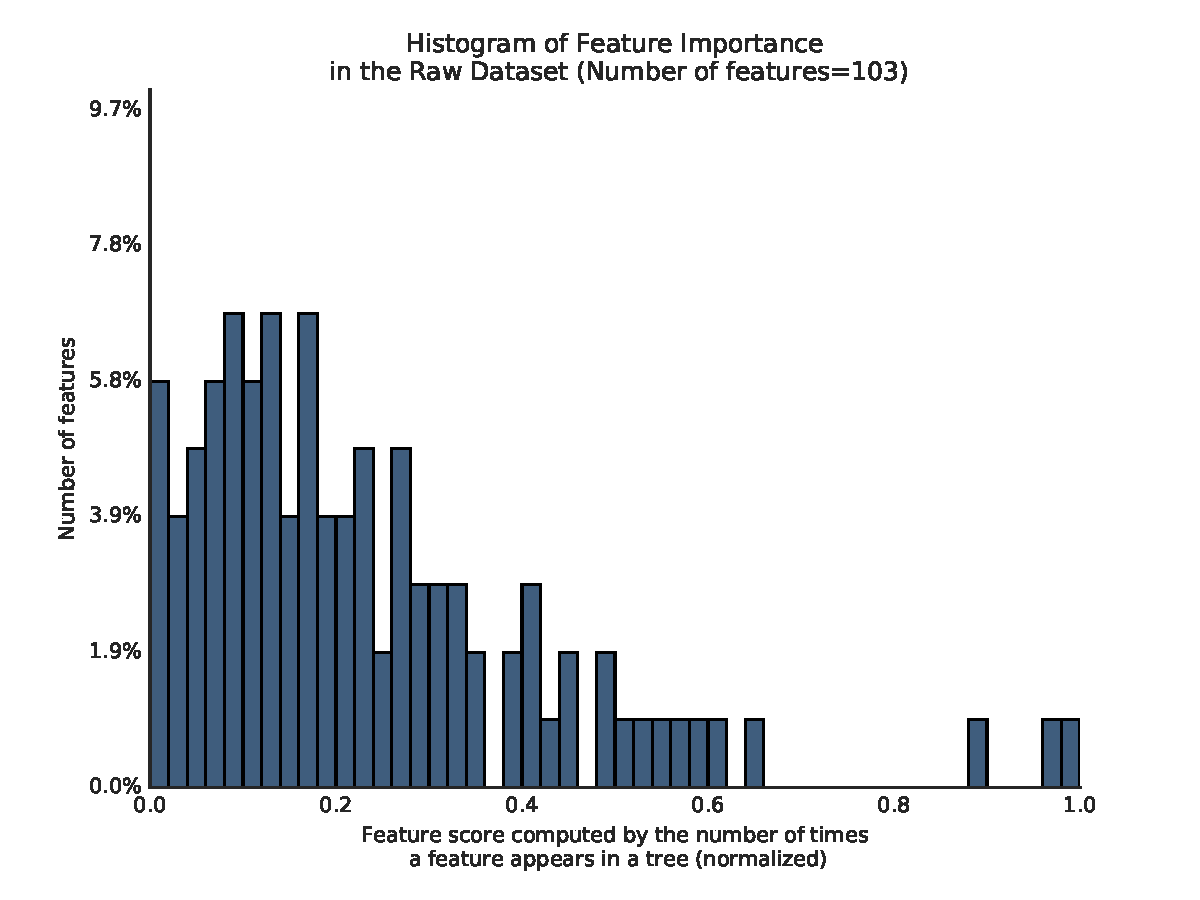
\includegraphics[width=\textwidth]{ch04/fi/fi_yeast_base}
        \caption{Yeast}
        \label{results:fi_yeast_base}
    \end{subfigure}
    ~ %add desired spacing between images, e. g. ~, \quad, \qquad, \hfill etc. 
      %(or a blank line to force the subfigure onto a new line)
    \begin{subfigure}[b]{0.45\textwidth}
        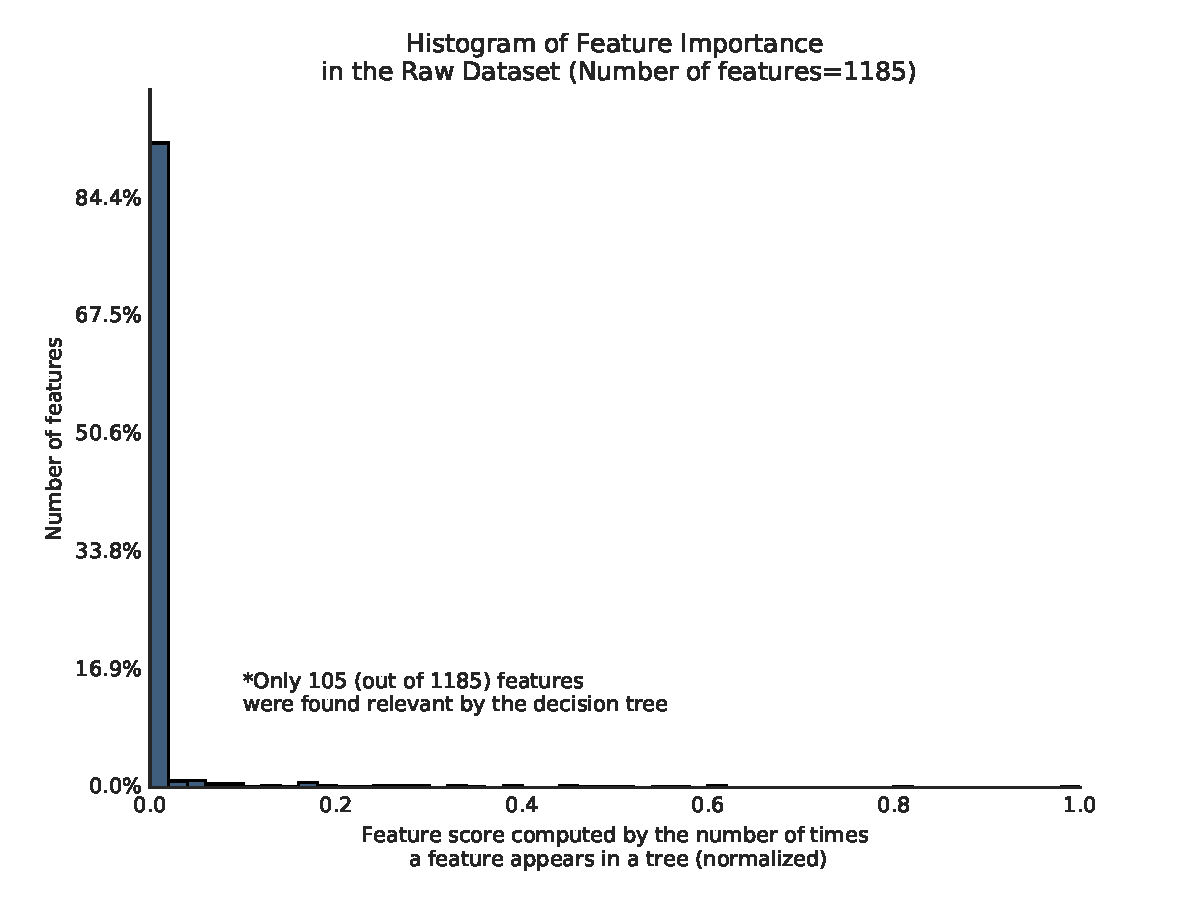
\includegraphics[width=\textwidth]{ch04/fi/fi_genbase_base}
        \caption{Genbase}
        \label{results:fi_genbase_base}
    \end{subfigure}
    \caption{Feature importance histogram for the raw data in both datasets}
    \label{results:fi_base}
\end{figure}

\begin{figure}[h!]
    \centering
    \begin{subfigure}[b]{0.45\textwidth}
        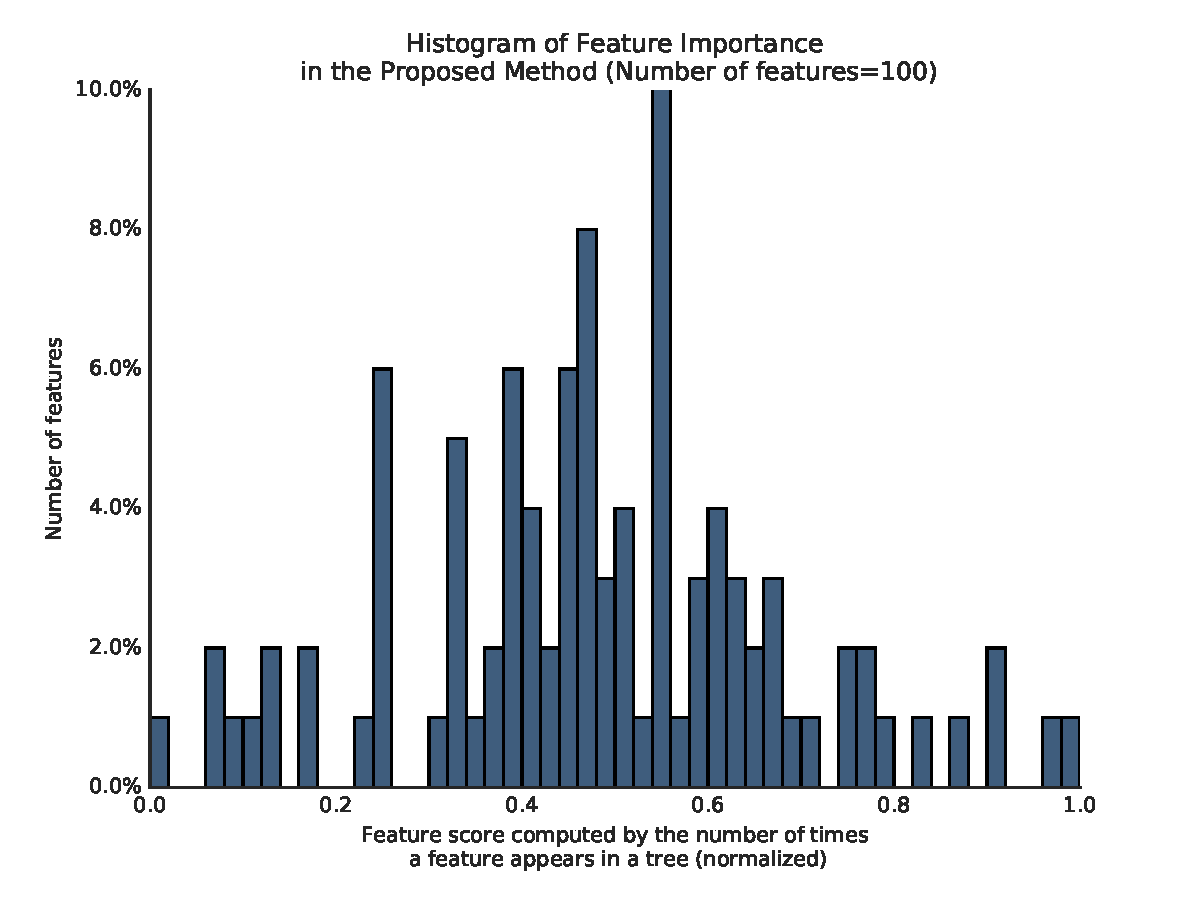
\includegraphics[width=\textwidth]{ch04/fi/fi_yeast_100}
        \caption{Number of features: $100$}
        \label{results:fi_yeast_100}
    \end{subfigure}
    ~ %add desired spacing between images, e. g. ~, \quad, \qquad, \hfill etc. 
      %(or a blank line to force the subfigure onto a new line)
    \begin{subfigure}[b]{0.45\textwidth}
        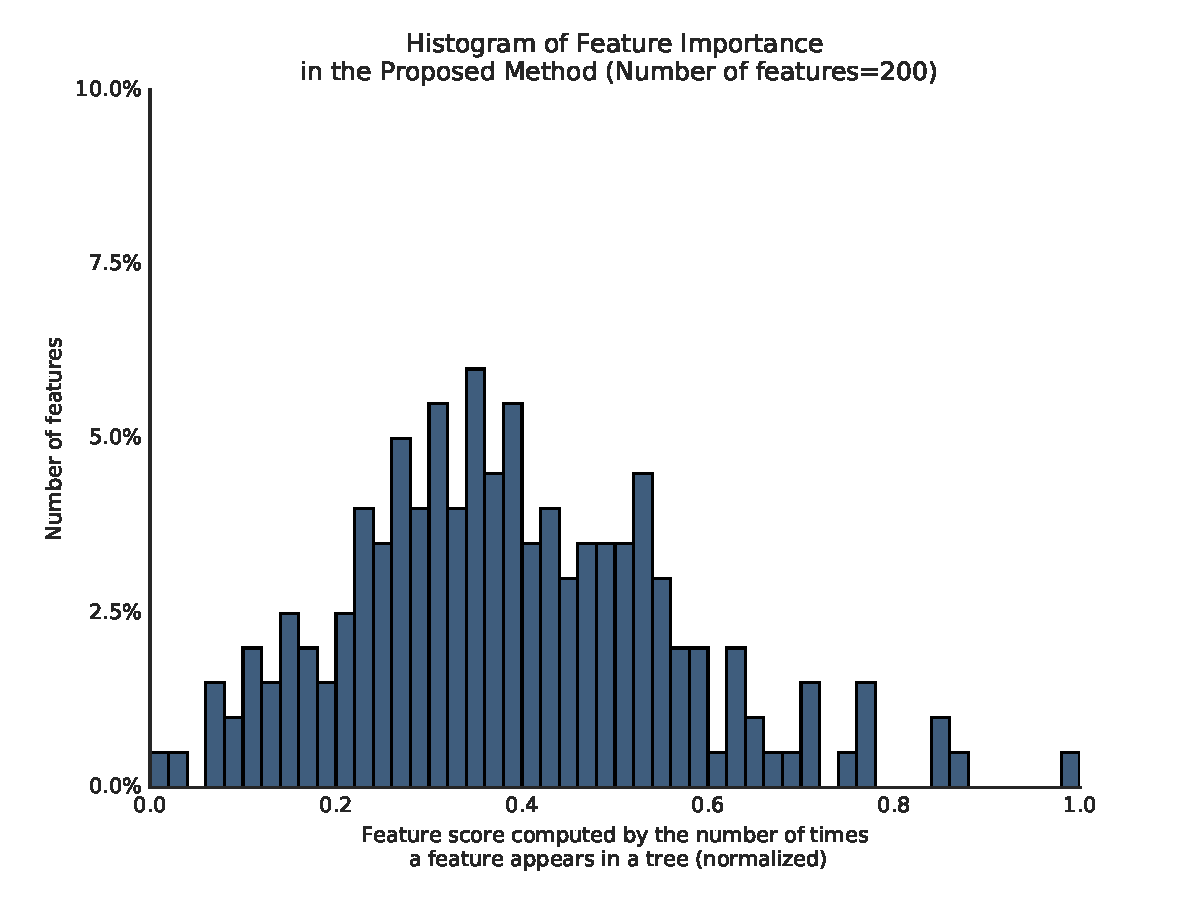
\includegraphics[width=\textwidth]{ch04/fi/fi_yeast_200}
        \caption{Number of features: $200$}
        \label{results:fi_yeast_200}
    \end{subfigure}
    ~ %add desired spacing between images, e. g. ~, \quad, \qquad, \hfill etc. 
      %(or a blank line to force the subfigure onto a new line)
    \begin{subfigure}[b]{0.45\textwidth}
        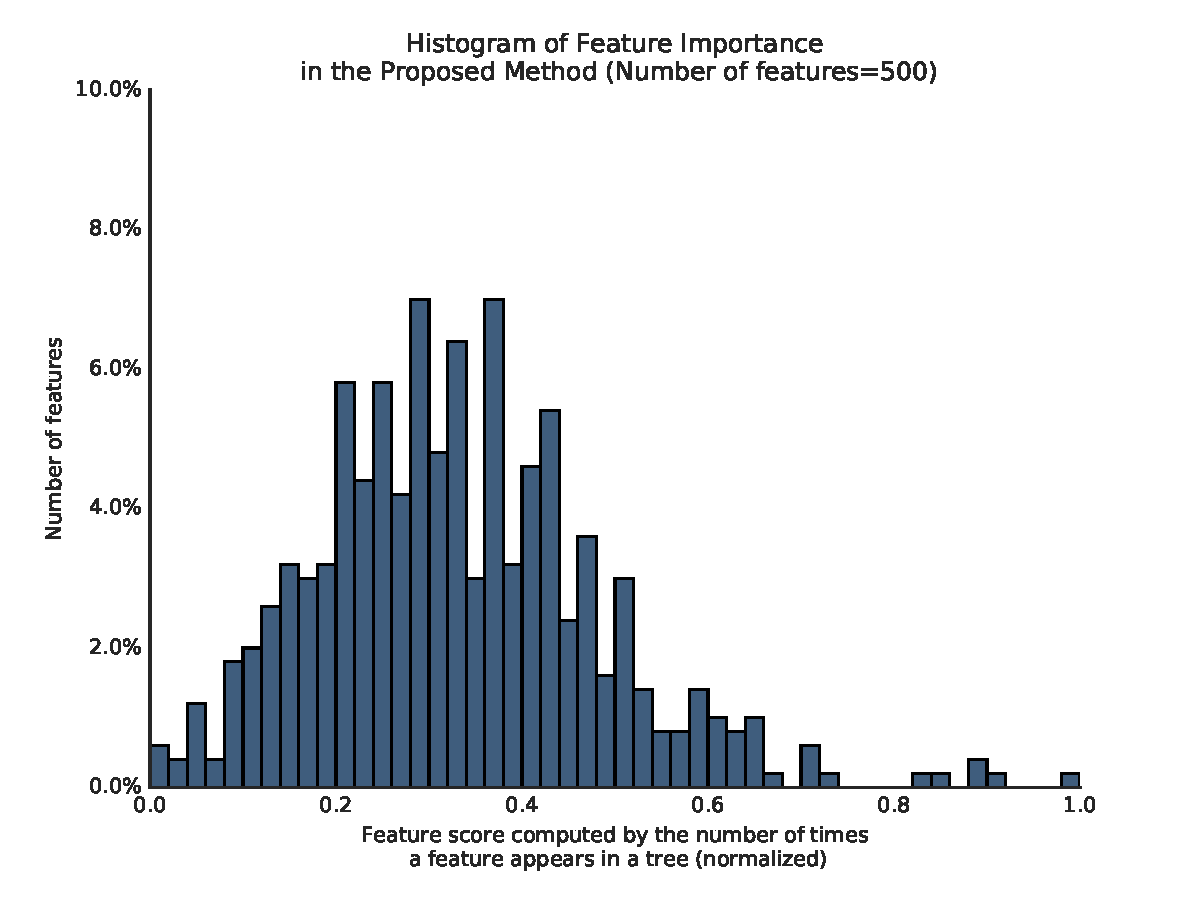
\includegraphics[width=\textwidth]{ch04/fi/fi_yeast_500}
        \caption{Number of features: $500$}
        \label{results:fi_yeast_500}
    \end{subfigure}
    ~ %add desired spacing between images, e. g. ~, \quad, \qquad, \hfill etc. 
      %(or a blank line to force the subfigure onto a new line)
    \begin{subfigure}[b]{0.45\textwidth}
        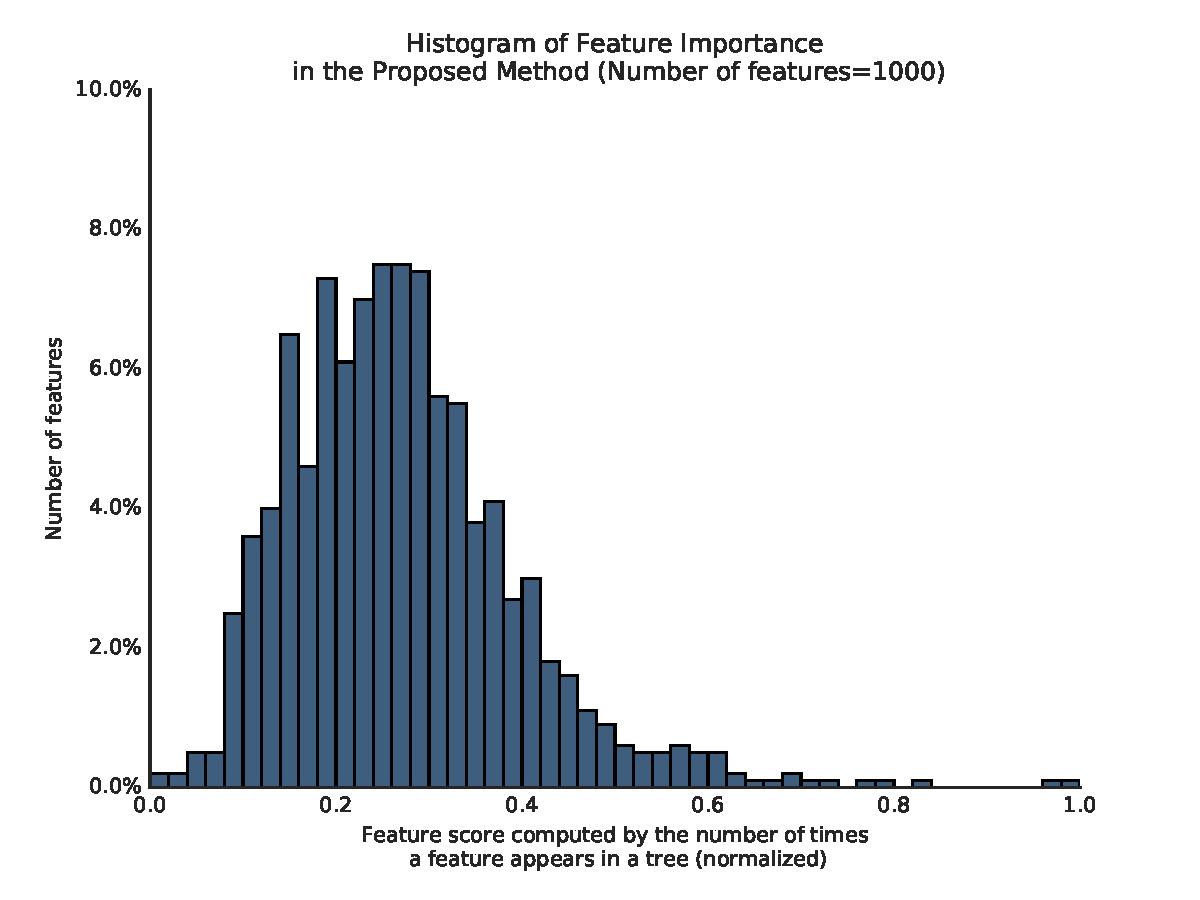
\includegraphics[width=\textwidth]{ch04/fi/fi_yeast_1000}
        \caption{Number of features: $1000$}
        \label{results:fi_yeast_1000}
    \end{subfigure}
    \caption{Feature importance histogram for the extracted features in Yeast}
    \label{results:fi_yeast}
\end{figure}

\paragraph{Yeast} The raw features tend to produce a left-leaning histogram
as shown in Figure \ref{results:fi_yeast_base}.  On the other hand, the score
distribution for the extracted features in Figure \ref{results:fi_yeast} have
moved into a higher range of scores. Interestingly, peaks are more noticeable
in lower dimensions, suggesting that relevant features are being extracted
while leaving others trivial. For higher dimensions, the distribution becomes
smoother. 

\begin{figure}[t]
    \centering
    \begin{subfigure}[b]{0.45\textwidth}
        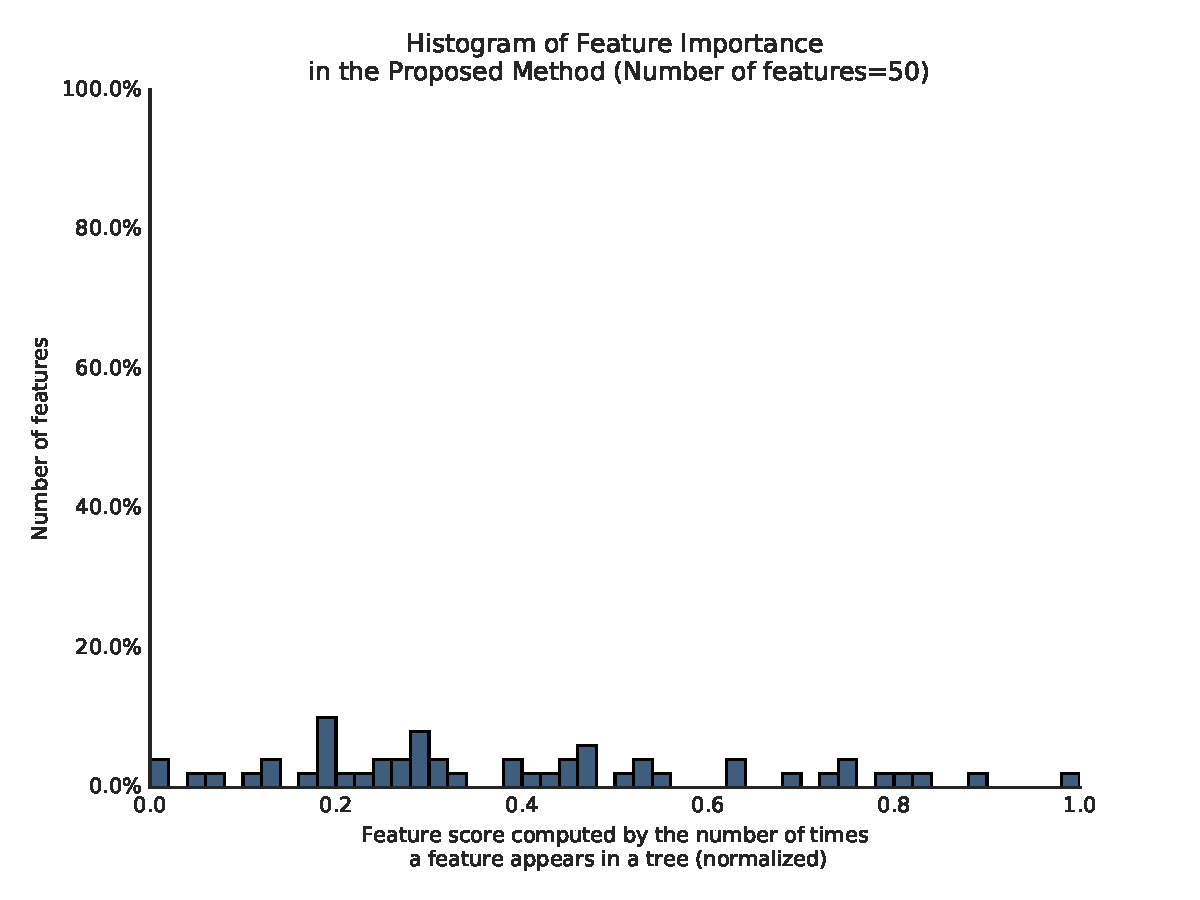
\includegraphics[width=\textwidth]{ch04/fi/fi_genbase_50}
        \caption{Number of features: $50$}
        \label{results:fi_genbase_50}
    \end{subfigure}
    ~ %add desired spacing between images, e. g. ~, \quad, \qquad, \hfill etc. 
      %(or a blank line to force the subfigure onto a new line)
    \begin{subfigure}[b]{0.45\textwidth}
        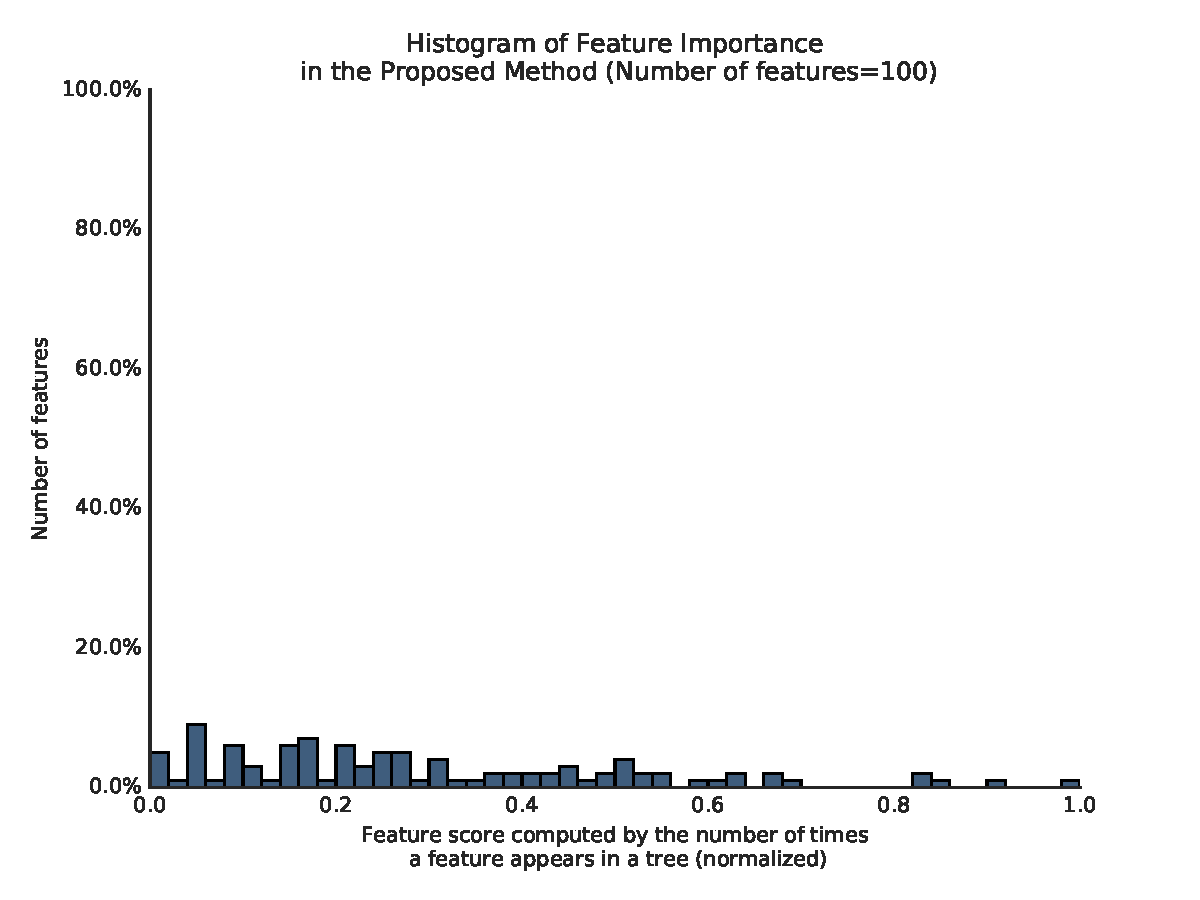
\includegraphics[width=\textwidth]{ch04/fi/fi_genbase_100}
        \caption{Number of features: $100$}
        \label{results:fi_genbase_100}
    \end{subfigure}
    ~ %add desired spacing between images, e. g. ~, \quad, \qquad, \hfill etc. 
      %(or a blank line to force the subfigure onto a new line)
    \begin{subfigure}[b]{0.45\textwidth}
        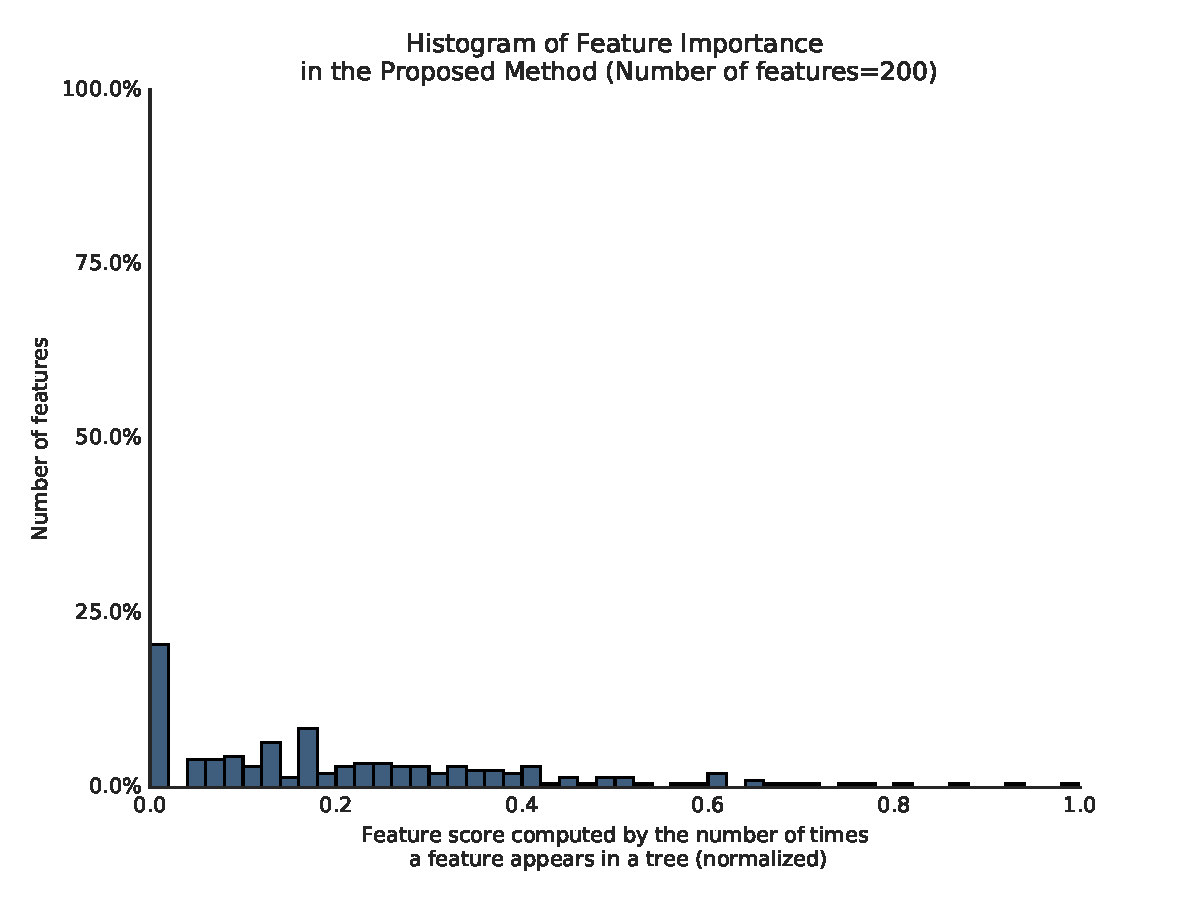
\includegraphics[width=\textwidth]{ch04/fi/fi_genbase_200}
        \caption{Number of features: $200$}
        \label{results:fi_genbase_200}
    \end{subfigure}
    ~ %add desired spacing between images, e. g. ~, \quad, \qquad, \hfill etc. 
      %(or a blank line to force the subfigure onto a new line)
    \begin{subfigure}[b]{0.45\textwidth}
        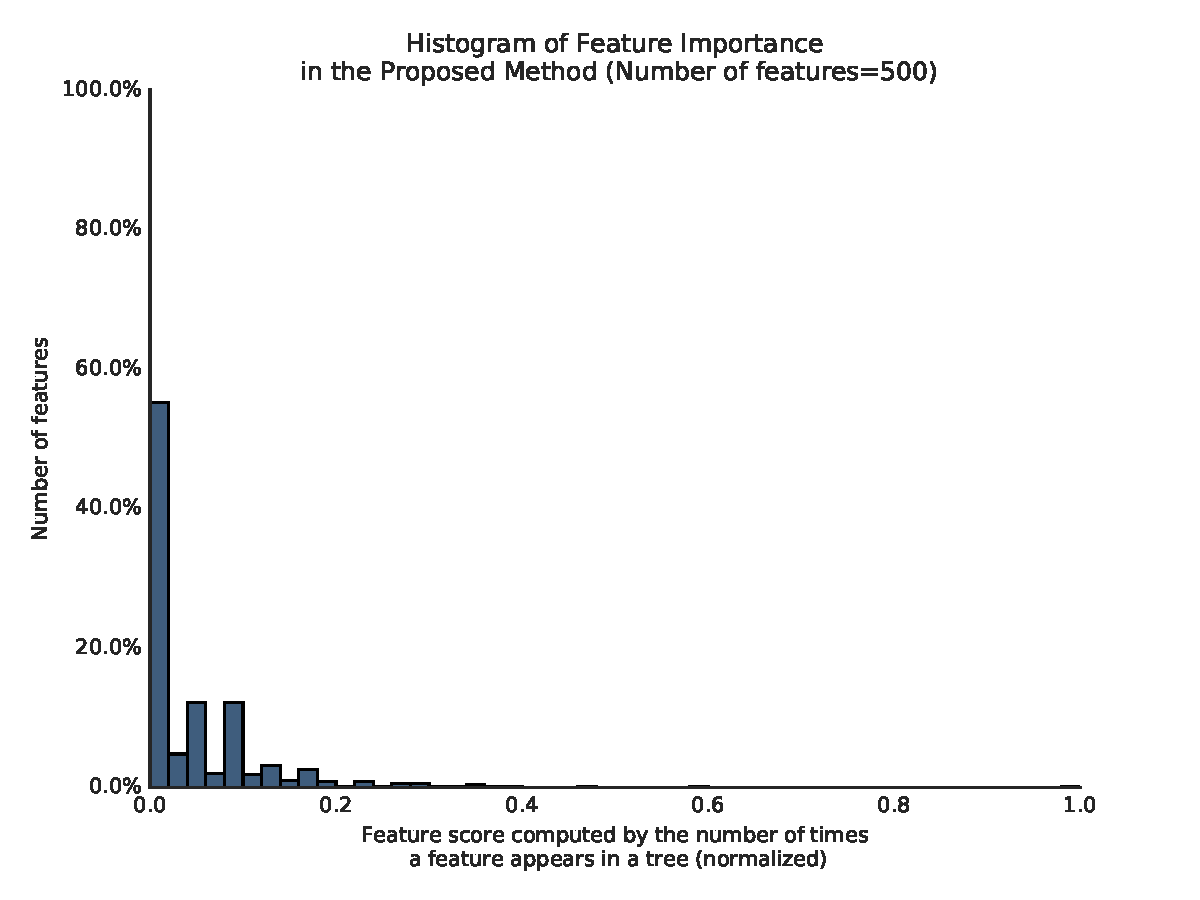
\includegraphics[width=\textwidth]{ch04/fi/fi_genbase_500}
        \caption{Number of features: $500$}
        \label{results:fi_genbase_500}
    \end{subfigure}
    \caption{Feature importance histogram for the extracted features in Genbase}
    \label{results:fi_genbase}
\end{figure}

\paragraph{Genbase} The histogram from \ref{results:fi_genbase_base} shows a
large number of the original feature set deemed irrelevant by the
decision-tree, as evidenced by the tall spike in the $0.0$ range. This suggests
that the features render the classification task more challenging. Compared
with the extracted features' scores in Figure \ref{results:fi_genbase}, the
distribution consists of more relevant features. The spike observed from the
raw inputs is not evident anymore (except in Fig.
\ref{results:fi_genbase_500}).\\

\par In summary, this experiment enables us to qualitatively observe how the
proposed method affects feature importance.  It is assumed that relevant
features boost classification, therefore helpful optimizing this
characteristic. By comparing feature score distribution across the whole
dataset, we can gauge feature relevance. From the experimental results, the
proposed method demonstrates the ability to extract more relevant features: the
score distribution of the new representations lie on the higher range in
contrast to the raw input. Next, we will investigate if feature relevance
indeed translates to better classification performance by measuring the quality
of the protein function prediction model.

\newpage
\section{Measuring model quality}
\label{ModelQuality}

\par This experiment enables us to gauge model performance in the two datasets.
Receiver operating characteristic (ROC) and precision-recall (PR) curves will
be drawn to accomplish this task. The ROC curve describes the sensitivity (true
positive rate) of the model as a function of its specificity (false positive
rate)\footnote[2]{In practice, we plot against $(1-\text{specificity})$} whereas
the PR curve illustrates the tradeoff between precision and recall for
different cutoff points. For both curves, a micro-average of all labels
will be plotted together with five (5) random classes in the labelset.

\begin{figure}[t]
    \centering
    \begin{subfigure}[b]{0.45\textwidth}
        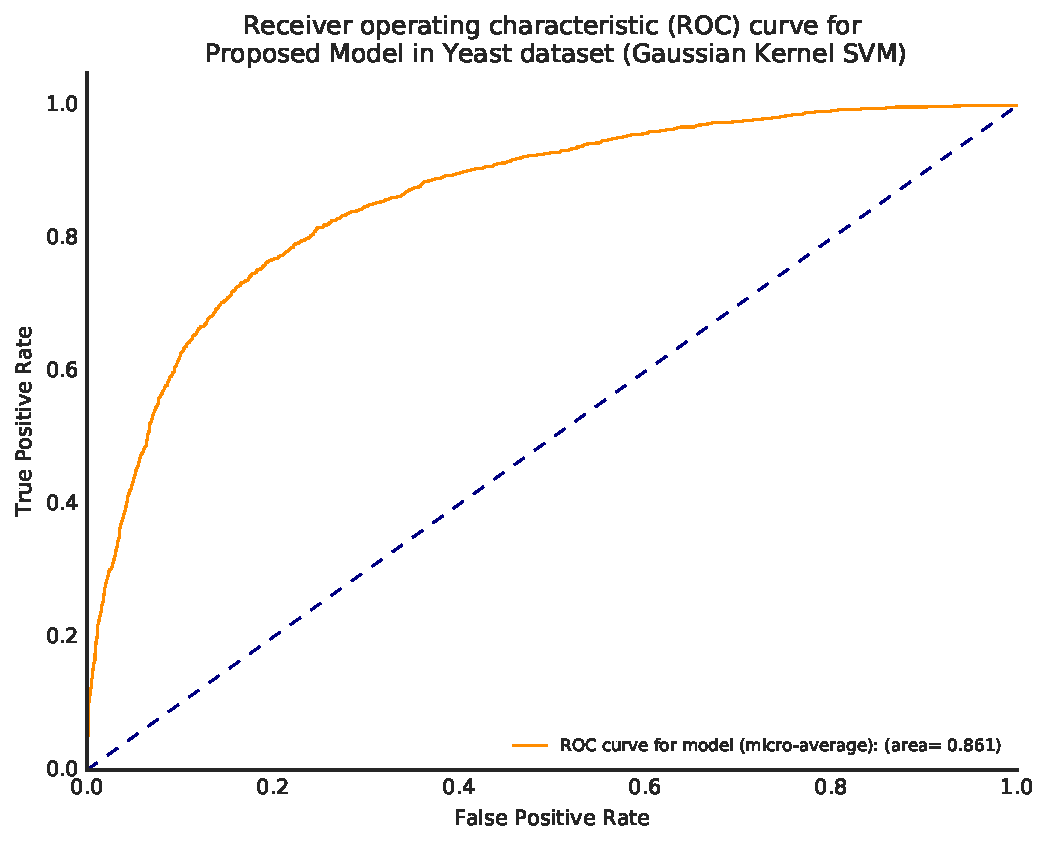
\includegraphics[width=\textwidth]{ch04/roc/roc_yeast_main}
        \caption{Micro-averaged across all labels}
        \label{results:roc_yeast_main}
    \end{subfigure}
    ~ %add desired spacing between images, e. g. ~, \quad, \qquad, \hfill etc. 
      %(or a blank line to force the subfigure onto a new line)
    \begin{subfigure}[b]{0.45\textwidth}
        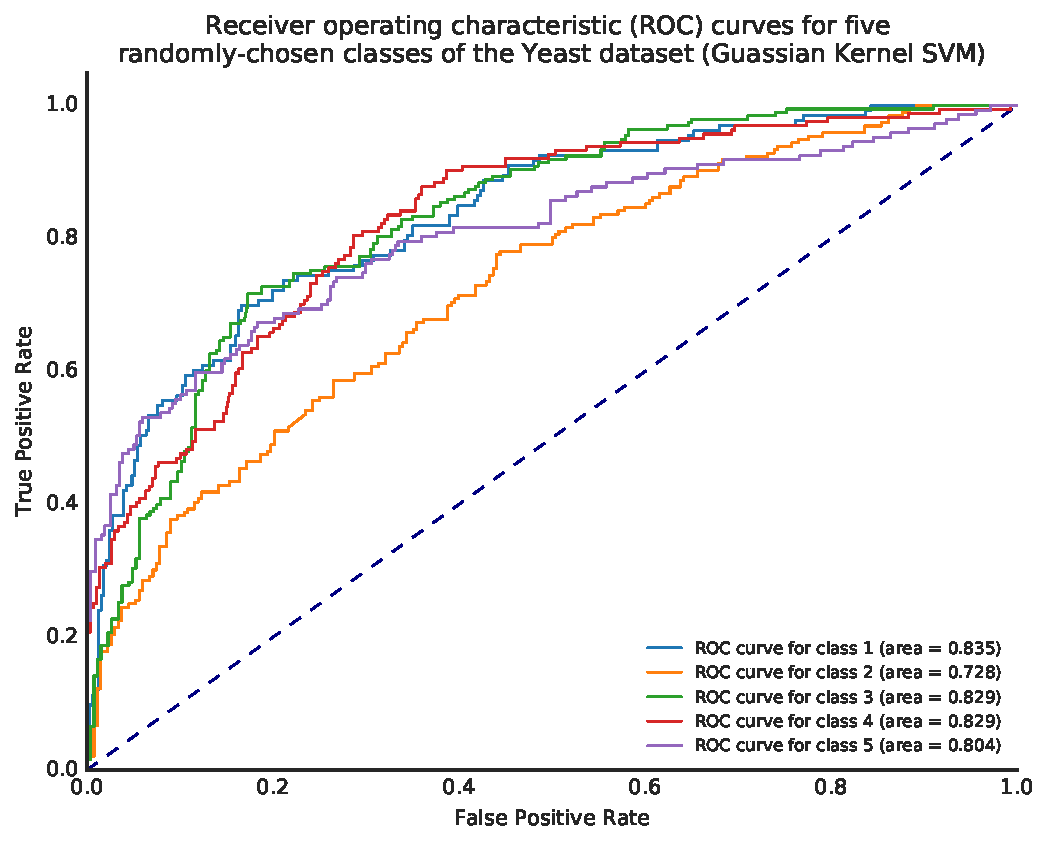
\includegraphics[width=\textwidth]{ch04/roc/roc_yeast_multiclass}
        \caption{Individual curves for five random labels}
        \label{results:roc_yeast_multiclass}
    \end{subfigure}
    \caption{Receiver Operating Characteristic (ROC) curves for the Yeast
    Dataset}
    \label{results:roc_yeast}
\end{figure}


\begin{figure}[t]
    \centering
    \begin{subfigure}[b]{0.45\textwidth}
        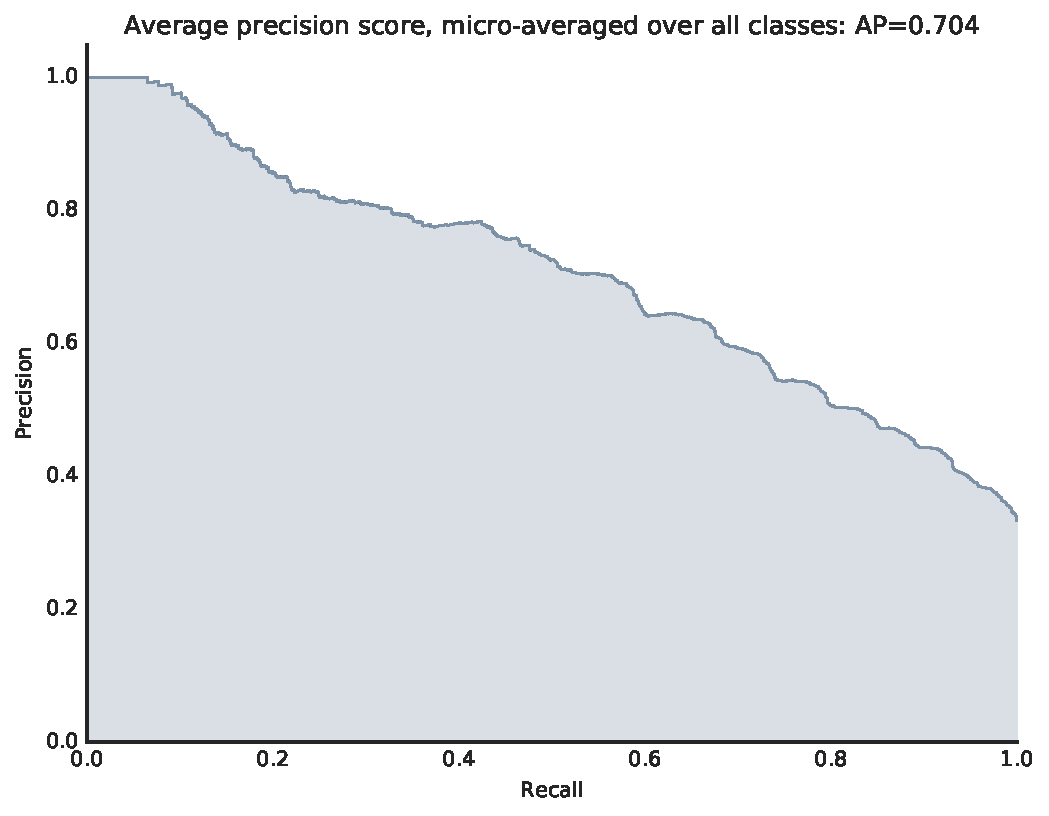
\includegraphics[width=\textwidth]{ch04/pr/pr_yeast_main}
        \caption{Micro-averaged across all labels}
        \label{results:pr_yeast_main}
    \end{subfigure}
    ~ %add desired spacing between images, e. g. ~, \quad, \qquad, \hfill etc. 
      %(or a blank line to force the subfigure onto a new line)
    \begin{subfigure}[b]{0.45\textwidth}
        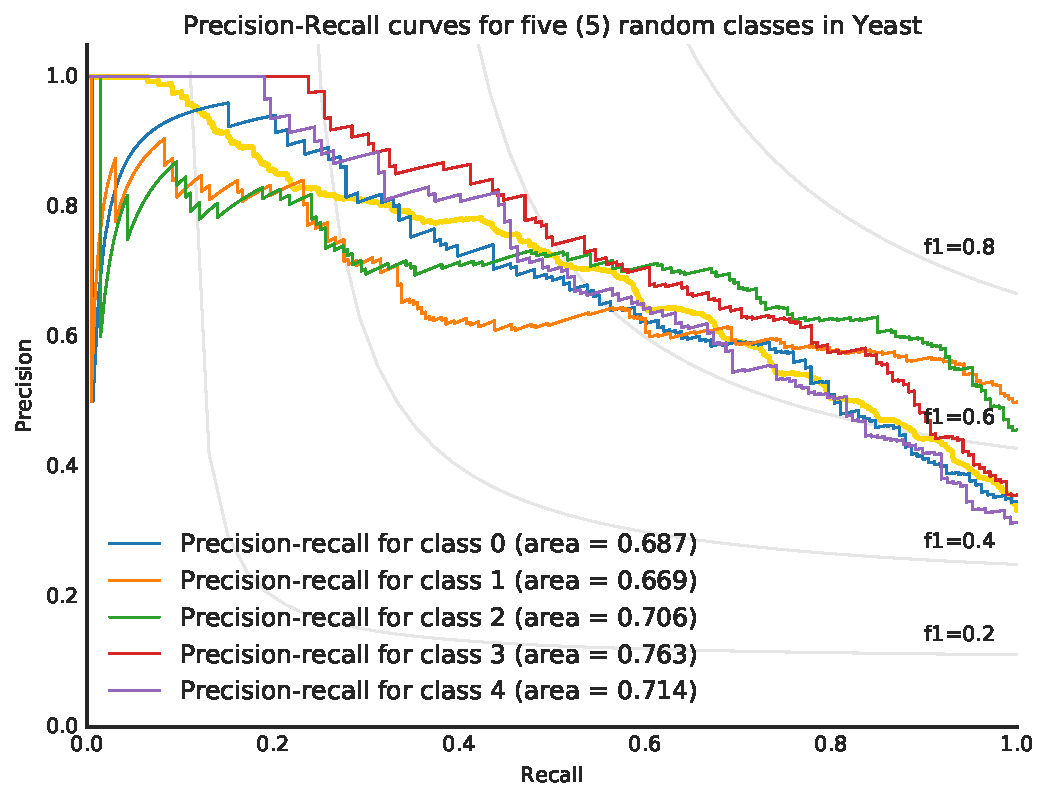
\includegraphics[width=\textwidth]{ch04/pr/pr_yeast_multi}
        \caption{Individual curves for five random labels}
        \label{results:pr_yeast_multi}
    \end{subfigure}
    \caption{Precision-Recall (PR) curves for the Yeast dataset}
    \label{results:pr_yeast}
\end{figure}

\paragraph{Yeast} Figure \ref{results:roc_yeast_main} shows that the model has
better performance than the baseline, given its large area under the curve
(i.e., $0.861$). In addition, the curves on Fig.
\ref{results:roc_yeast_multiclass} also have relatively large areas under it,
indicating that the quality is well-distributed to different labels. Lastly,
the PR curves in Fig.  \ref{results:pr_yeast} show an estimated F-score in the
range of $0.5$ to $0.7$, and can still be improved by tuning the
hyperparameters.

\paragraph{Genbase} For this dataset, the model tends to perform well as
evidenced by the $0.995$ performance in Figure \ref{results:roc_genbase_main}.
This is also well-distributed to different classes as evidenced by Fig.
\ref{results:roc_genbase_multiclass}. Lastly, the PR-curves show conformation to
this quality, showing a good score even for different classes.  \\ 


\begin{figure}[t]
    \centering
    \begin{subfigure}[b]{0.45\textwidth}
        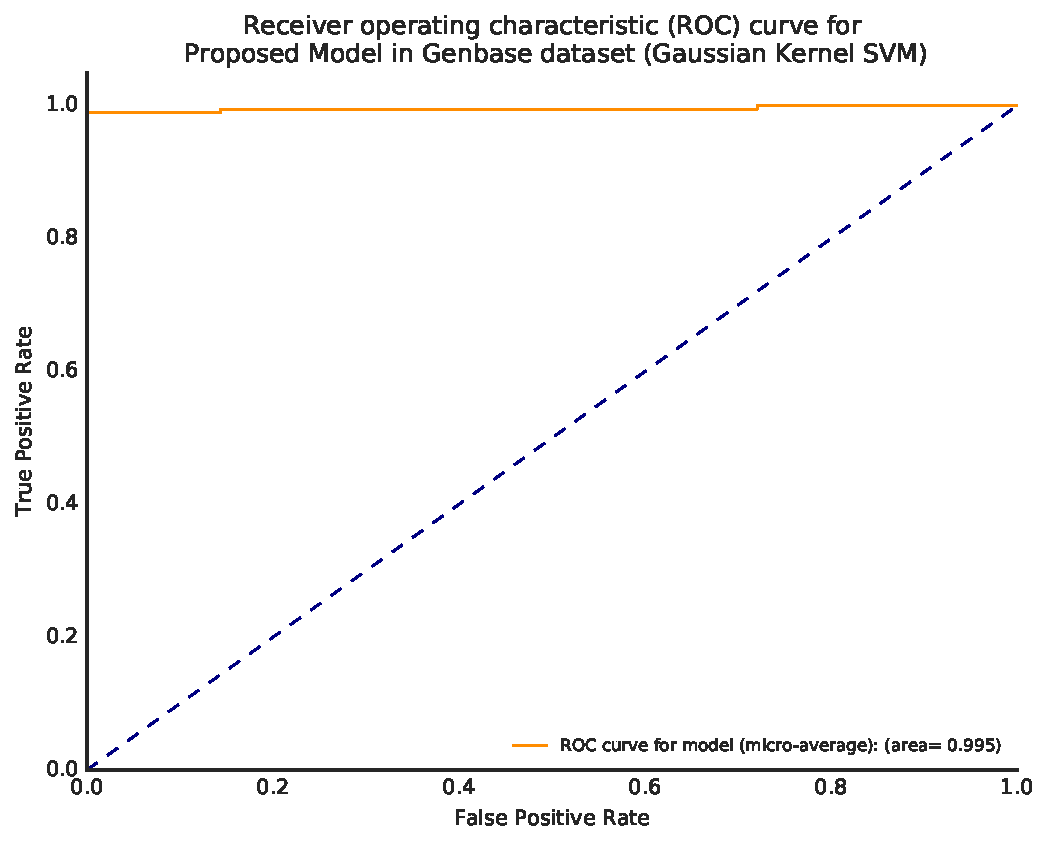
\includegraphics[width=\textwidth]{ch04/roc/roc_genbase_main}
        \caption{Micro-averaged across all labels}
        \label{results:roc_genbase_main}
    \end{subfigure}
    ~ %add desired spacing between images, e. g. ~, \quad, \qquad, \hfill etc. 
      %(or a blank line to force the subfigure onto a new line)
    \begin{subfigure}[b]{0.45\textwidth}
        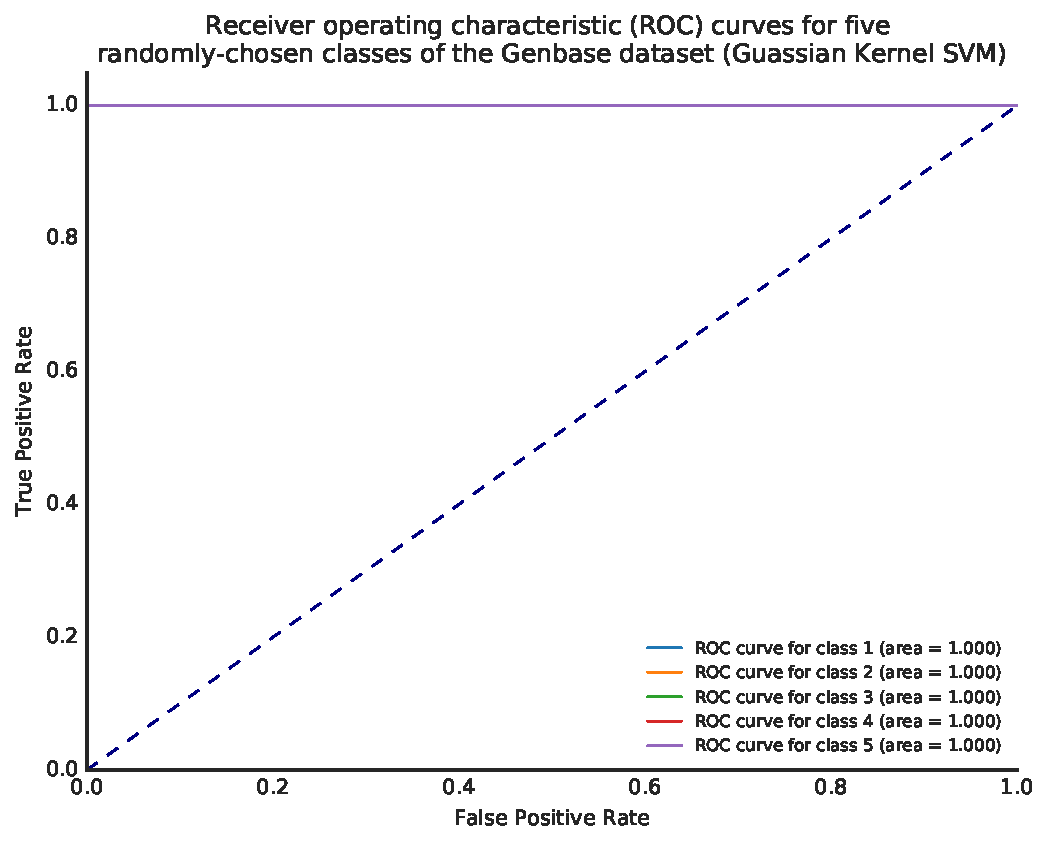
\includegraphics[width=\textwidth]{ch04/roc/roc_genbase_multiclass}
        \caption{Individual curves for five random labels}
        \label{results:roc_genbase_multiclass}
    \end{subfigure}
    \caption{Receiver Operating Characteristic (ROC) curves for the Genbase
    Dataset}
    \label{results:roc_genbase}
\end{figure}


\begin{figure}[t]
    \centering
    \begin{subfigure}[b]{0.45\textwidth}
        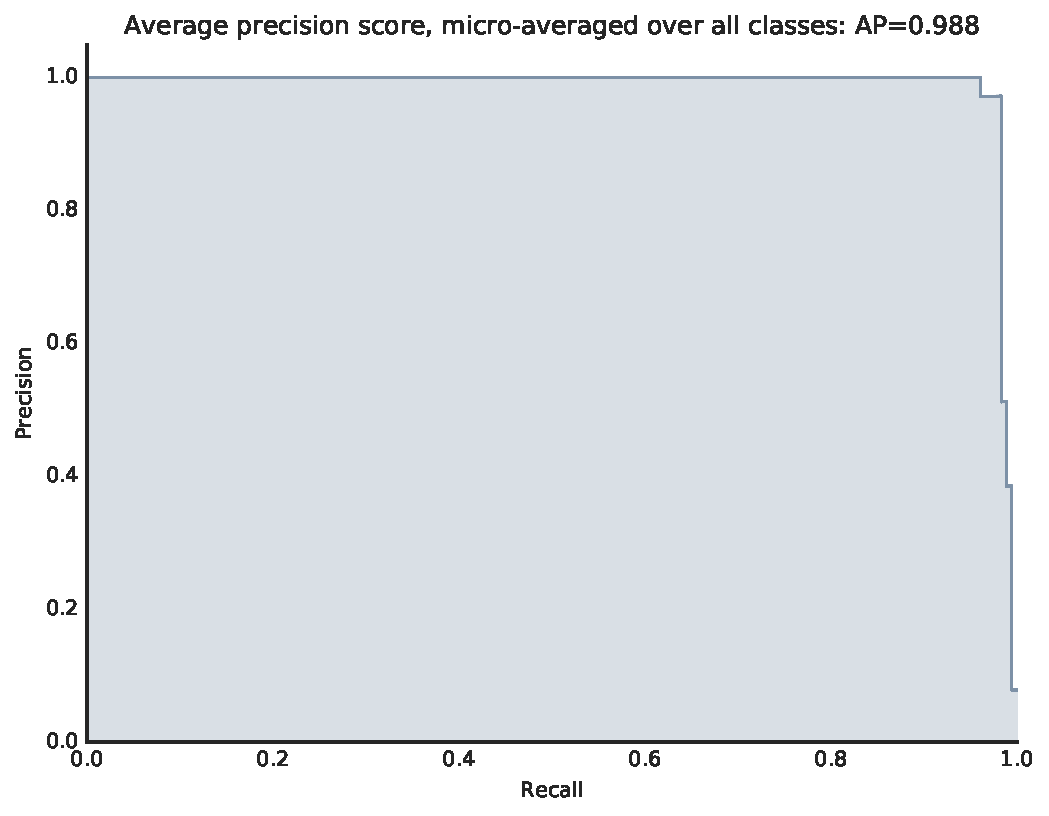
\includegraphics[width=\textwidth]{ch04/pr/pr_genbase_main}
        \caption{Micro-averaged across all labels}
        \label{results:pr_genbase_main}
    \end{subfigure}
    ~ %add desired spacing between images, e. g. ~, \quad, \qquad, \hfill etc. 
      %(or a blank line to force the subfigure onto a new line)
    \begin{subfigure}[b]{0.45\textwidth}
        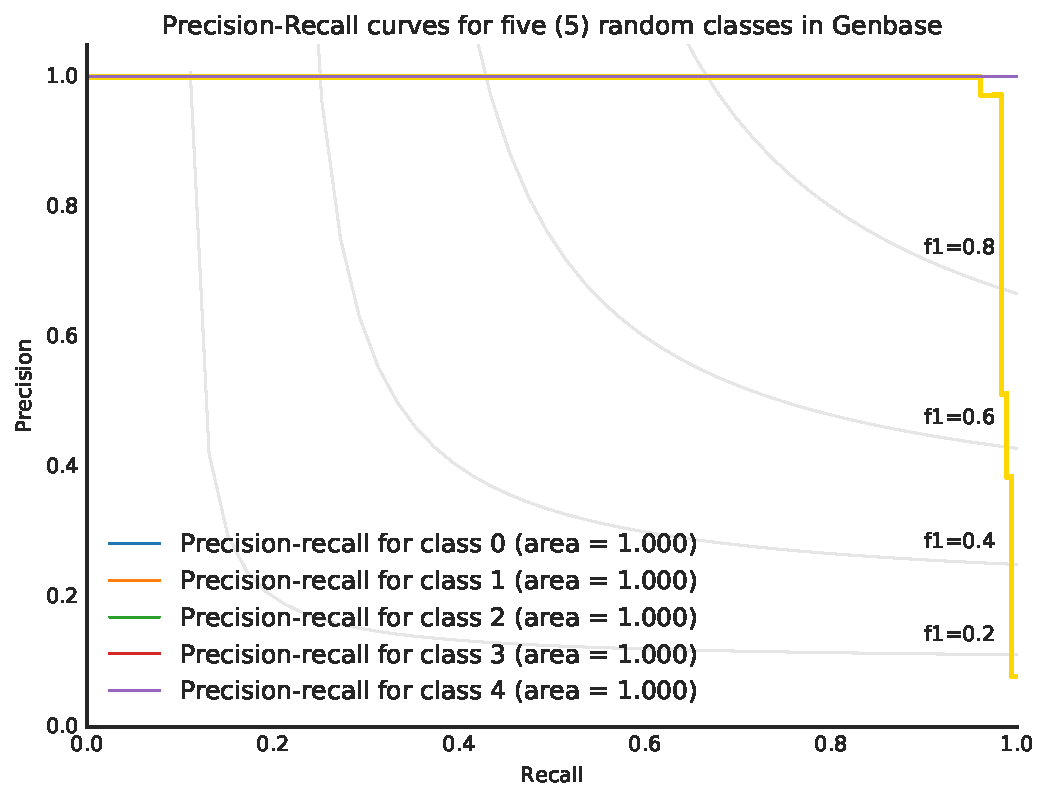
\includegraphics[width=\textwidth]{ch04/pr/pr_genbase_multi}
        \caption{Individual curves for five random labels}
        \label{results:pr_genbase_multi}
    \end{subfigure}
    \caption{Precision-Recall (PR) curves for the Genbase dataset}
    \label{results:pr_genbase}
\end{figure}

\par Lastly, Table \ref{results:pr_table} gives the precision and recall
measurements for the model using two different SVM kernels and three averaging
methods. It is evident that using the Gaussian kernel for SVM works in favor to
improve model performance. In addition, the results are relatively decent and
can still be improved by hyperparameter tuning.

\begin{table}[!ht]
    \centering
    \caption{Average precision and recall for both datasets}
    \label{results:pr_table}
    \begin{tabular}{@{}lrllcll@{}}
    \toprule
     &         & \multicolumn{5}{c}{Dataset}                             \\ \cmidrule{3-7}
     &         & \multicolumn{2}{c}{Yeast} &\phantom{abc} & \multicolumn{2}{c}{Genbase} \\ \cmidrule{3-4} \cmidrule{6-7}
     &                      & Linear     & Gaussian  && Linear    & Gaussian  \\ \midrule
\multicolumn{2}{l}{Precision} \\
     & \textit{micro}       & 0.538191   & 0.639692  &&  0.988006 & 0.973023  \\
     & \textit{macro}       & 0.569659   & 0.648473  &&  0.980438 & 0.988342  \\
     & \textit{samples}     & 0.545558   & 0.648483  &&  0.994149 & 0.982895  \\
\multicolumn{2}{l}{Recall} \\
     & \textit{micro}       & 0.577003   & 0.618419  &&  0.986286 & 1.000000  \\
     & \textit{macro}       & 0.577003   & 0.618419  &&  0.986286 & 1.000000  \\
     & \textit{samples}     & 0.583777   & 0.636325  &&  0.991726 & 1.000000  \\ \bottomrule
    \end{tabular}
\end{table}


\par In summary, the ROC and PR curves gave insights on model performance for
the two datasets. From the experimental results, the proposed model delivered
higher performance compared to the baseline\textemdash  defined as a classifier
with area under ROC of $0.5$. In addition, the PR curves also demonstrated a
good precision-recall tradeoff for both datasets. However, model quality cannot
easily be judged in isolation. For the next set of experiments, we will put
model performance into context by benchmarking it against other techniques in
literature. 

\section{Comparison to other models}
\label{Benchmarking}

\par In this section, the proposed model will be compared to other works in
literature. The existing works follow the same pipeline for protein function
prediction\textemdash extract features from data, then classify with the
extracted features:

\begin{itemize}
    \item \cite{wang2013protein} applied principal component
    analysis (PCA) to reduce the dimensions of protein data from $353$ to
    $204$. 
    \item \cite{chicco2014deep} used a deep autoencoder with two-layers
    to predict the protein functions of \textit{B.taurus} and \textit{G.
    gallus}. 
    \item \cite{miranda2017feature} implemented a stacked denoising
    autoencoder to obtain robust features from raw data to predict protein
    functions.  
\end{itemize}

\par In addition, we will also compare against a baseline model without feature
extraction. All features, extracted or not, will be trained on a
binary-relevance SVM for classification with both gaussian and linear kernels.
The trained model then predicts the samples from a held-out test set.  The
entire pipeline will run for ten (10) trials with the mean and standard
deviation reported. Tables \ref{results:yeast_svm} to \ref{results:genbase_lsvm}
show the outcome for the two datasets using different SVM kernels.

\par The top performer is highlighted in bold font for each criteria: the
highest value for AUROC and F-score and the lowest for Hamming loss. Overall,
the proposed method outperformed all other techniques in literature including
the baseline. However, to fully assess our model's performance, statistical
tests of significance are implemented.

\subsection{Statistical tests of significance}

To assess if the performance of the proposed model is significant against other
techniques, two statistical tests were employed: Friedman's test
and a post-hoc Nemenyi test. The Friedman's test determines if the results across all
methods are significantly different. If difference is detected, then a post-hoc
Nemenyi test checks for significant difference in each method against the proposed
model \footnote[2]{Friedman's test asks the following question: are methods A,
B, C different from one another? If they are, then a post-hoc Nemenyi test will
ask: is method A significantly different to method B? to method C? and so on.}.
These tests were recommended by \cite{demsar2006statistical}  and was patterned
from most literature reviews in multilabel learning
(\cite{madjarov2012extensive, zhang2014review}). 

\par For the Friedman's test, the null hypothesis $H_{0}$ states that there is no
significant difference across all methods. Comparing the computed
$\chi^{2}$ statistic and $p$-value, we can reject $H_{0}$ at different
confidence level $\alpha$ as summarized in Table
\ref{results:friedman}. At the same time, the test can be performed at
different levels of comparison: (i) across each dataset and classifier, (ii)
across datasets, (iii) overall. From the test results, it is evident that
there is significant difference among the models' performance.Thus we can
proceed to a post-hoc test.

\par Because all datasets passed the Friedman's test, a post-hoc Nemenyi test
can be implemented to check the proposed model's performance against other
methods. Here, the null hypothesis $H_{0}$ states that there is no
significant difference between two methods A and B. Table
\ref{results:nemenyi} shows the results when comparing each method across
datasets and overall. 

\begin{table}[!ht]
    \footnotesize
    \centering
    \caption{Results for the Yeast Dataset using SVM with Gaussian Kernel}
    \label{results:yeast_svm}
    \begin{threeparttable}
    \begin{tabular}{@{}rrlllll@{}}
    \toprule
    && \multicolumn{5}{c}{Prediction Model} \\ \cmidrule{3-7}
    \multicolumn{2}{r}{Metrics}               & Baseline                & Wang, 2013 & Chicco, 2014 & Miranda, 2017 & Proposed            \\ \midrule
\multicolumn{2}{l}{Area ROC} \\
                    & \textit{micro}            & $0.6668 \pm 0.0031$ & $0.6559 \pm 0.0020$ & $0.6430 \pm 0.0012$ & $0.6679 \pm 0.0025$ & $\mathbf{0.7320 \pm 0.0021} $ \\
                     & \textit{macro}            & $0.6548 \pm 0.0031$ & $0.6590 \pm 0.0024$ & $\mathbf{0.6624 \pm 0.0011}$ & $0.6484 \pm 0.0022$ & $0.6455 \pm 0.0018 $ \\
                     & \textit{samples}            & $0.6700 \pm 0.0032$ & $0.6559 \pm 0.0019$ & $0.6443 \pm 0.0011$ & $0.6569 \pm 0.0026$ & $\mathbf{0.7433 \pm 0.0040} $ \\
\multicolumn{2}{l}{F-score} \\
                    & \textit{micro}            & $0.5483 \pm 0.0041$ & $0.5381 \pm 0.0023$ & $0.5304 \pm 0.0014$ & $0.5792 \pm 0.0028$ & $\mathbf{0.6289 \pm 0.0024} $ \\
                     & \textit{macro}            & $0.5970 \pm 0.0035$ & $0.6033 \pm 0.0024$ & $0.5896 \pm 0.0011$ & $0.6132 \pm 0.0023$ & $\mathbf{0.6299 \pm 0.0024} $ \\
                     & \textit{samples}            & $0.5359 \pm 0.0032$ & $0.5242 \pm 0.0022$ & $0.5171 \pm 0.0014$ & $0.5720 \pm 0.0034$ & $\mathbf{0.6086 \pm 0.0038} $ \\ 
\multicolumn{2}{l}{Hamm. Loss}            & $0.3222 \pm 0.0021$ & $0.3430 \pm 0.0018$ & $0.3535 \pm 0.0011$ & $0.2310 \pm 0.0031$ & $\mathbf{0.2241 \pm 0.0019}$ \\
\bottomrule
    \end{tabular}
    \begin{tablenotes}
        \item SVM Hyperparameters for Proposed Model: $C=1.000$, $\gamma=1.67e-3$
    \end{tablenotes}
    \end{threeparttable}
\end{table}

\begin{table}[t]
    \footnotesize
    \centering
    \caption{Results for the Yeast Dataset using SVM with Linear Kernel}
    \label{results:yeast_lsvm_main}
    \begin{threeparttable}
    \begin{tabular}{@{}lllllll@{}}
    \toprule
    \multicolumn{2}{l}{Metrics}      & Base                 & PCA                  & AE                  & SdAE          & Proposed      \\ \midrule
    H     & \textit{--}               & $0.3507 \pm 0.0012$  & $0.3619  \pm 0.0021$ & $0.3739 \pm 0.0005$ & $0.3170 \pm 0.0036$ & $\mathbf{0.2794 \pm 0.0053}$ \\
    A     & \textit{mi}              & $0.6504 \pm 0.0021$  & $0.6465 \pm 0.0022$  & $0.6287 \pm 0.0005$ & $0.6425 \pm 0.0022$ & $\mathbf{0.6802 \pm 0.0071}$ \\
          & \textit{ma}              & $0.6507 \pm 0.0016$  & $\mathbf{0.6548 \pm 0.0016}$  & $0.6524 \pm 0.0009$ & $0.6099 \pm 0.0013$ & $0.6012 \pm 0.0072$ \\
          & \textit{sp}              & $0.6525 \pm 0.0022$  & $0.6499 \pm 0.0023$  & $0.6299 \pm 0.0005$ & $0.6471 \pm 0.0019$ & $\mathbf{0.6851 \pm 0.0079}$ \\
    F     & \textit{mi}              & $0.5330 \pm 0.0032$  & $0.5305 \pm 0.0025$  & $0.5173 \pm 0.0006$ & $0.5445 \pm 0.0024$ & $\mathbf{0.5569 \pm 0.0097}$ \\
          & \textit{ma}              & $0.5913 \pm 0.0031$  & $\mathbf{0.6023 \pm 0.0019}$  & $0.5816 \pm 0.0006$ & $0.5779 \pm 0.0019$ & $0.5709 \pm 0.0094$ \\
          & \textit{sp}              & $0.5223 \pm 0.0031$  & $0.5217 \pm 0.0027$  & $0.5101 \pm 0.0008$ & $0.5302 \pm 0.0020$ & $\mathbf{0.5354 \pm 0.0107}$ \\ \bottomrule
    \end{tabular}
    \begin{tablenotes}
      \item SVM Hyperparameters for Proposed Model: $C=3.594$
    \end{tablenotes}
   \end{threeparttable}
\end{table}


\begin{table}[h!]
    \footnotesize
    \centering
    \caption{Results for the Genbase Dataset using SVM with Gaussian Kernel}
    \label{results:genbase_svm}
    \begin{threeparttable}
    \begin{tabular}{@{}rrlllll@{}}
    \toprule
    && \multicolumn{5}{c}{Prediction Model} \\ \cmidrule{3-7}
    \multicolumn{2}{r}{Metrics}               & Baseline                & Wang, 2013 & Chicco, 2014 & Miranda, 2017 & Proposed            \\ \midrule
\multicolumn{2}{l}{Area ROC} \\
           & \textit{micro}       & $0.8563 \pm 0.0002$ & $0.9872 \pm 0.0001$ &
$0.9741 \pm 0.0098$ & $0.9872 \pm 0.0009$ & $\mathbf{0.9992 \pm 0.0000}$ \\
            & \textit{macro}       & $0.6706 \pm 0.0004$ & $0.9928 \pm 0.0002$
            & $0.9786 \pm 0.0106$ & $0.9834 \pm 0.0009$ & $\mathbf{0.9996 \pm
            0.0000}$ \\
            & \textit{samples}       & $0.6129 \pm 0.0003$ & $0.9503 \pm
0.0001$ & $0.9756 \pm 0.0097$ & $0.9875 \pm 0.0007$ & $\mathbf{0.9992 \pm
0.0000}$ \\
\multicolumn{2}{l}{F-score} \\
           & \textit{micro}       & $0.6706 \pm 0.0003$ & $0.8872 \pm 0.0008$ &
$0.7846 \pm 0.0865$ & $0.9619 \pm 0.0109$ & $\mathbf{0.9863 \pm 0.0070}$ \\
            & \textit{macro}       & $0.7159 \pm 0.0005$ & $0.9503 \pm 0.0002$
            & $0.8922 \pm 0.0400$ & $0.9640 \pm 0.0061$ & $\mathbf{0.9919 \pm
            0.0020}$ \\
            & \textit{samples}       & $0.7603 \pm 0.0001$ & $0.9282 \pm 0.0004$ & $0.8098 \pm 0.0945$ & $0.9699 \pm 0.0080$ & $\mathbf{0.9886 \pm 0.0063}$ \\ 
    \multicolumn{2}{l}{Hamm. Loss} & $0.0407 \pm 0.0001$ & $0.0141 \pm 0.0021$
                                   & $0.0352 \pm 0.0168$ & $0.0045 \pm 0.0013$
                                   & $\mathbf{0.0016 \pm 0.0000}$ \\ \bottomrule
    \end{tabular}
    \begin{tablenotes}
        \item SVM Hyperparameters for Proposed Model: $C=1.000$, $\gamma=1.24e-3$
    \end{tablenotes}
    \end{threeparttable}
    \end{table}

\begin{table}[!ht]
    \footnotesize
    \centering
    \caption{Results for the Genbase Dataset using SVM with Linear Kernel}
    \label{results:genbase_lsvm}
    \begin{threeparttable}
        \begin{tabular}{@{}rrlllll@{}}
        \toprule
    && \multicolumn{5}{c}{Prediction Model} \\ \cmidrule{3-7}
    \multicolumn{2}{r}{Metrics}               & Baseline                & Wang, 2013 & Chicco, 2014 & Miranda, 2017 & Proposed            \\ \midrule
\multicolumn{2}{l}{Area ROC} \\
                   & \textit{micro}       & $0.9779 \pm 0.0079$ & $0.9782 \pm 0.0015$ & $0.9493 \pm 0.0165$ & $0.9926 \pm 0.0014$ & $\mathbf{0.9928 \pm 0.0019}$ \\
                    & \textit{macro}       & $0.9770 \pm 0.0010$ & $0.9876 \pm 0.0013$ & $0.9628 \pm 0.0151$ & $\mathbf{0.9936 \pm 0.0004}$ & $0.9929 \pm 0.0019$ \\
                    & \textit{samples}       & $0.9795 \pm 0.0015$ & $0.9796 \pm 0.0013$ & $0.9515 \pm 0.0165$ & $0.9948 \pm 0.0013$ & $\mathbf{0.9955 \pm 0.0010}$ \\
\multicolumn{2}{l}{F-score} \\
                   & \textit{micro}       & $0.7495 \pm 0.0023$ & $0.8074 \pm 0.0042$ & $0.6054 \pm 0.0884$ & $0.9671 \pm 0.0216$ & $\mathbf{0.9871 \pm 0.0034}$ \\
                    & \textit{macro}       & $0.8209 \pm 0.0081$ & $0.9198 \pm 0.0002$ & $0.7793 \pm 0.0581$ & $0.9757 \pm 0.0070$ & $\mathbf{0.9824 \pm 0.0033}$ \\
                    & \textit{samples}       & $0.8279 \pm 0.0088$ & $0.8474 \pm 0.0012$ & $0.6965 \pm 0.0711$ & $0.9732 \pm 0.0188$ & $\mathbf{0.9916 \pm 0.0022}$ \\ 
\multicolumn{2}{l}{Hamm. Loss}                & $0.0367 \pm 0.0041$ & $0.0263
\pm 0.0021$ & $0.0840 \pm 0.0309$ & $0.0038 \pm 0.0026$ & $\mathbf{0.0014 \pm
0.0004}$ \\ \bottomrule
        \end{tabular}
        \begin{tablenotes}
                \item SVM Hyperparameters for Proposed Model: $C=4.500$
        \end{tablenotes}
    \end{threeparttable}
    \end{table}


\par For the Yeast dataset, the proposed method's performance is not that
apparent against the $\textit{Baseline}$ and \cite{wang2013protein}, but are
significant against the two autoencoder models. For the Genbase dataset, the
proposed method's performance is not that significant against
\cite{miranda2017feature}, but are significant against all other techniques ($p
\leq 0.01$ and $p \leq 0.05$). Lastly, when accounting for overall performance,
the proposed method significantly performs better against other techniques in
literature ($p \leq 0.01$).

\par In summary, this set of experiments aims to determine how well the
proposed method performs against other techniques in literature. Test results
showed that the autoencoder with mutual competition performs significantly
better than the baseline and to other feature extraction methods. Overall, the
post-hoc Nemenyi test confirmed that the proposed model outperforms others in
the two classification tasks. This also showed that extracting features before
classification improves inference, as the model exceeds baseline performance.
Next, we will further test if the modifications to the basic autoencoder are
relevant by way of ablation. The proposed model will be built gradually,
adding one hyperparameter over the other to the basic autoencoder, while being
tested for AUROC.  

\begin{table}[t]
    \footnotesize
    \centering
    \caption{$p$-values for Friedman's test of significance}
    \label{results:friedman}
    \begin{threeparttable}
    \begin{tabular}{@{}llll@{}}
    \toprule
    Comparison                & $\chi^2$    & $p$-value       & Sig.\tnote{1}   \\ \midrule
    Yeast with Gaussian-SVM   & $13.257$    & $0.0101$        & **              \\
    Yeast with Linear-SVM     & $11.200$    & $0.0244$        & **              \\
    Genbase with Gaussian-SVM & $26.388$    & $2.642e-5$      & ***             \\
    Genbase with Linear-SVM   & $27.314$    & $1.717e-5$      & ***             \\ \cmidrule{1-4}
    Yeast                     & $18.400$    & $0.001031$      & ***             \\
    Genbase                   & $50.251$    & $3.201e-10$     & ***             \\ \cmidrule{1-4}
    Overall (all datasets)    & $47.335$    & $1.299e-09$     & ***             \\ \bottomrule
    \end{tabular}
    \begin{tablenotes}
        \item[1] Significance: * - $p \leq 0.1$, ** - $p \leq 0.05$, *** - $p \leq 0.01$
    \end{tablenotes}
    \end{threeparttable}
\end{table}

\begin{table}[t]
    \footnotesize
    \centering
    \caption{$p$-values from the post-hoc Nemenyi Test against the proposed method}
    \label{results:nemenyi}
    \begin{threeparttable}
    \begin{tabular}{@{}lllll@{}}
    \toprule
    Dataset                & Baseline    & Wang, 2013     & Chicco, 2014      &
    Miranda, 2017\\ \midrule
    Yeast                  & $0.8746 $ & $0.5273 $ & $0.0020^{***}$ & ${5.5e-05}^{***}$ \\
    Genbase                & ${9.6e-08}^{***}$ & $0.01335^{**}$ & ${1.9e-07}^{***}$ & $0.48859$ \\ \cmidrule{1-5}
    Overall (all datasets) & ${2.2e-05}^{***}$ & $0.00752^{***}$ & ${4.3e-10}^{***}$ & $0.00013^{***}$ \\ \bottomrule
    \end{tabular}
    \begin{tablenotes}
        \item Significance: * - $p \leq 0.1$, ** - $p \leq 0.05$, *** - $p \leq 0.01$
    \end{tablenotes}
    \end{threeparttable}
    \end{table}


\section{Ablation Tests}
\label{AblationTest}

\par Ablation testing checks if the modifications is necessary. The test starts
with a \textit{source configuration}, a default model that is widely used, and
is iteratively built to achieve the \textit{target configuration} or the
proposed model. In this experiment, we start with the basic autoencoder and
iteratively add two components\textemdash the winner-take-all (WTA) and sparse
operations (MC)\textemdash until we reach the proposed model. At the same time,
the area under the ROC curve (AUROC) for the test data will be recorded. Figure
\ref{results:ab_analysis} shows the test results for both datasets. It is
evident that the modifications made in the basic autoencoder model helped
improve model performance overall.   

\begin{figure}[h]
    \centering
    \begin{subfigure}[b]{0.45\textwidth}
        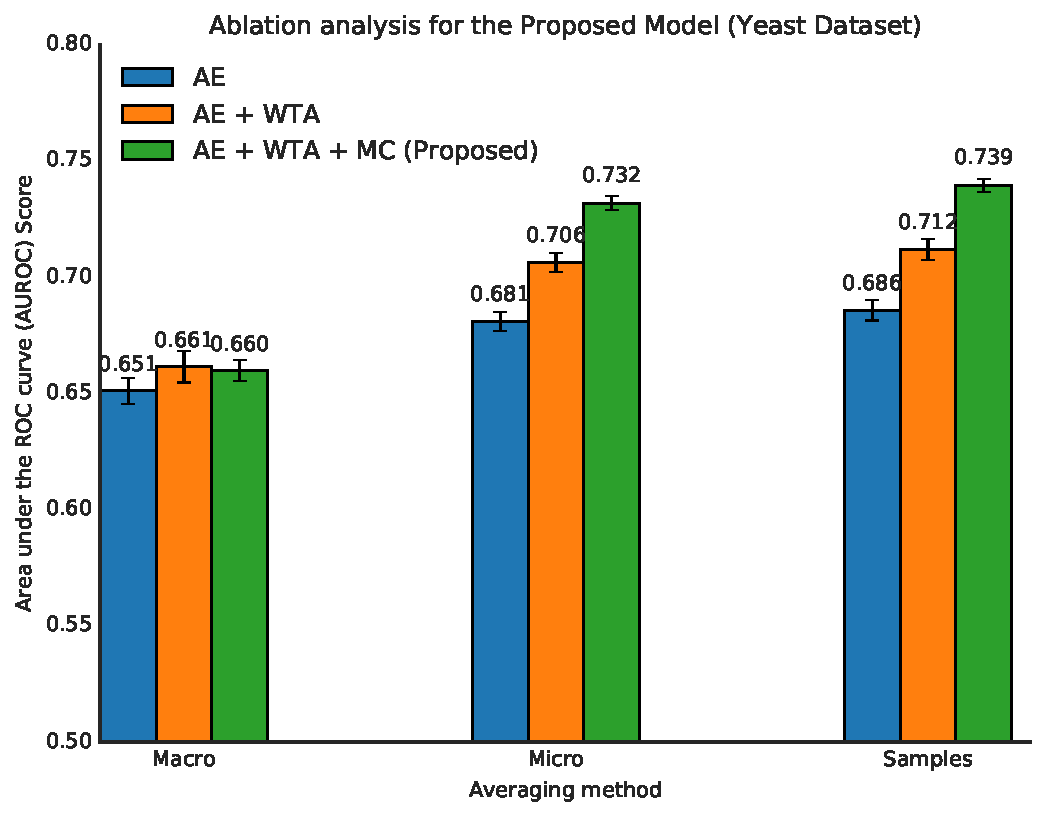
\includegraphics[width=\textwidth]{ch04/ab/ab_yeast}
        \caption{Yeast}
        \label{results:ab_yeast}
    \end{subfigure}
    ~ %add desired spacing between images, e. g. ~, \quad, \qquad, \hfill etc. 
      %(or a blank line to force the subfigure onto a new line)
    \begin{subfigure}[b]{0.45\textwidth}
        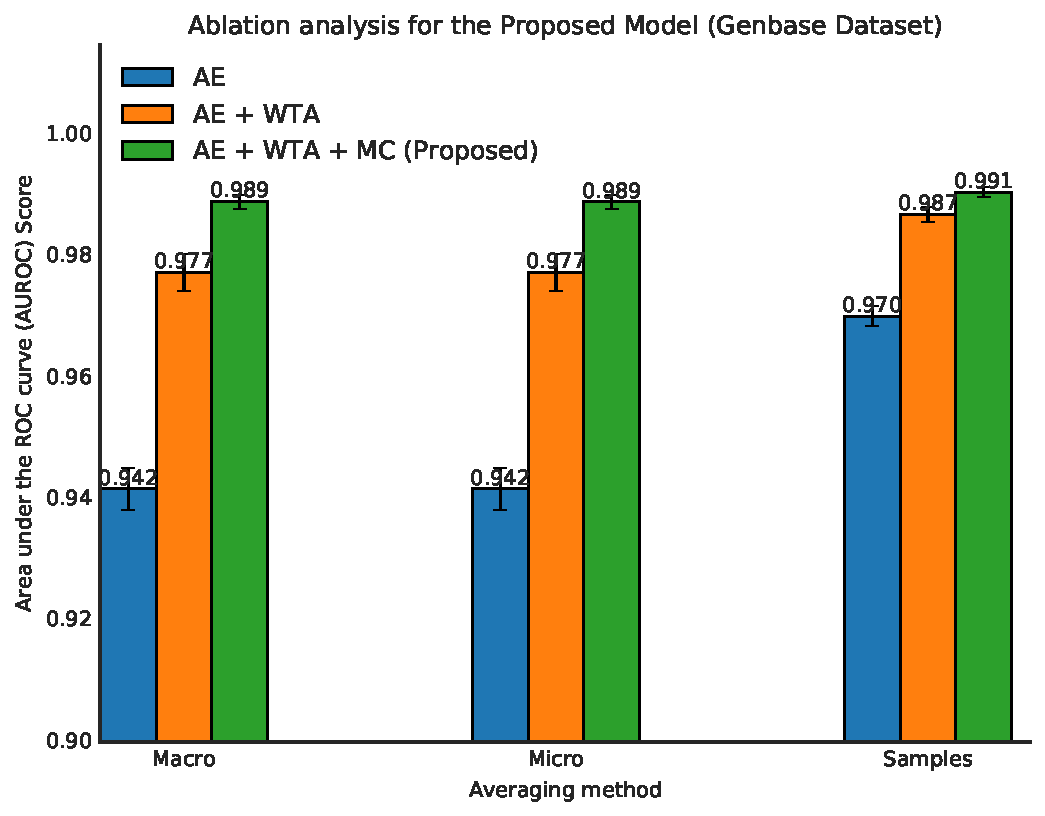
\includegraphics[width=\textwidth]{ch04/ab/ab_genbase}
        \caption{Genbase}
        \label{results:ab_genbase}
    \end{subfigure}
    \caption{Ablation analysis for both datasets}
    \label{results:ab_analysis}
\end{figure}
